\documentclass[border=10pt]{standalone}

\usepackage{tikz}
\usepackage{tikzsymbols}
\usetikzlibrary{calc,patterns,shapes.geometric}

\def\centerarc[#1](#2)(#3:#4:#5){\draw[#1] ($(#2)+({#5*cos(#3)},{#5*sin(#3)})$) arc (#3:#4:#5);}

\begin{document}
	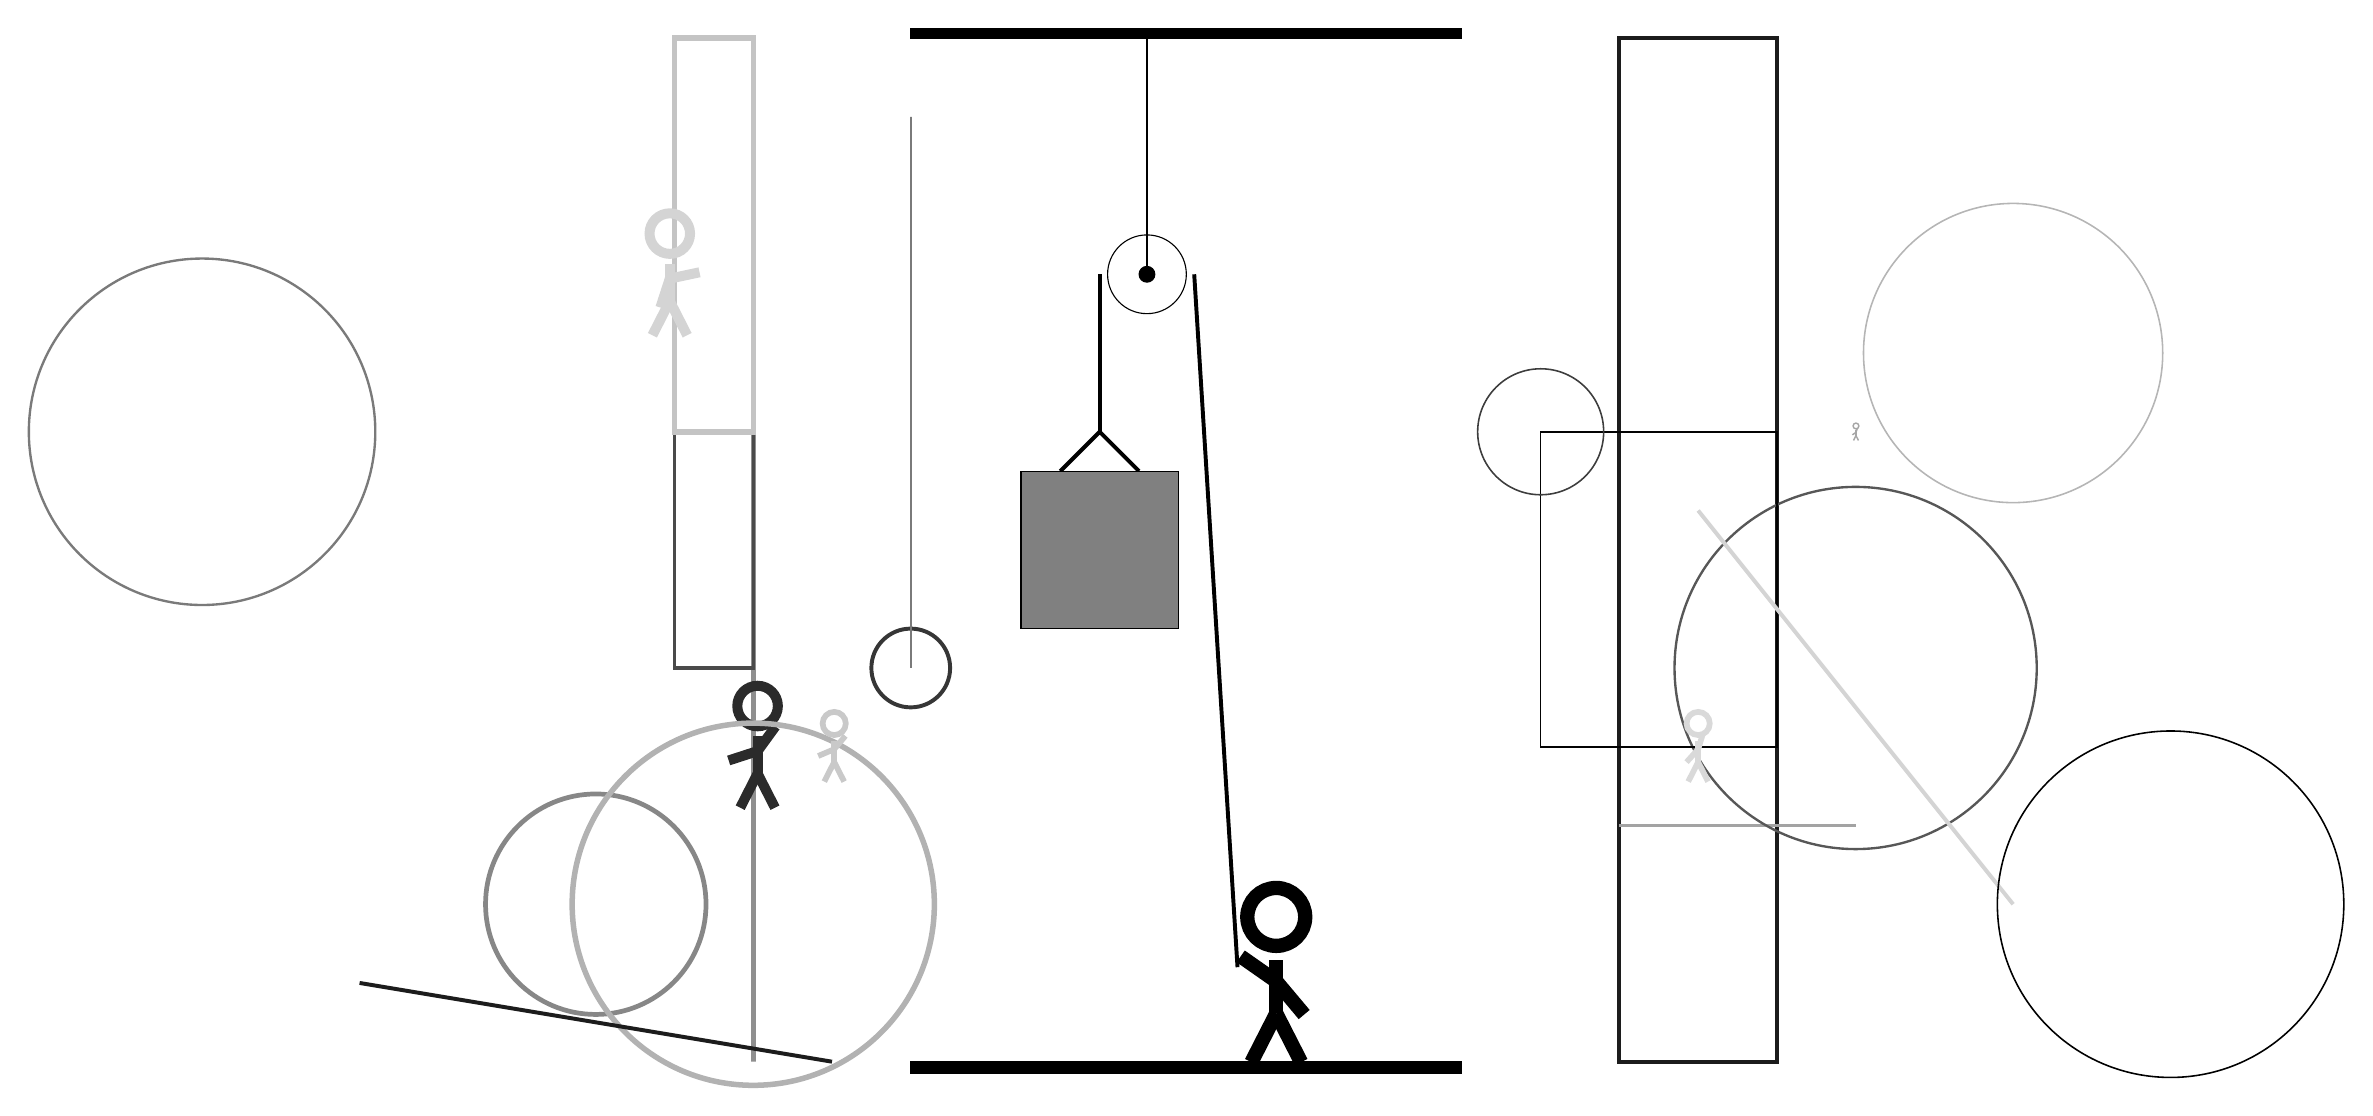
\begin{tikzpicture}
		%%%%% START %%%%%
		
		\draw[fill=black] (-2, 10) rectangle (5, 10.125);
		
		\draw (1, 7) circle (0.5);
		\draw[fill=black] (1, 7) circle (0.1);
		\draw (1, 10) -- (1, 7);
		
		\draw[line width=0.5mm] (-0.1, 4.5) -- (0.4, 5.0) -- (0.9, 4.5);
		\draw[fill=black!50] (-0.6, 4.5) rectangle (1.4, 2.5);
		
		\draw[line width=0.5mm] (0.4, 7) -- (0.4, 5.0);
		\centerarc[line width=0.5mm](1, 7)(0:180:0.6);
		\draw[line width=0.5mm](1.6, 7) -- (2.15, -1.8);
		
		\node at (2.6, -1.9) {\Strichmaxerl[10][-35][-50]};
		
		\draw[line width=0.5mm, color=black!89] (7, 10) rectangle (9, -3);
		
		\draw[line width=0.6mm, color=black!44] (-4, -3) rectangle (-4, 9);
		\draw[line width=0.5mm, color=black!36](10, 0) -- (7, 0);
		\draw [line width=0.6mm, color=black!47](-6, -1) circle (1.4);
		\draw[line width=0.4mm, color=black!71] (-4, 5) rectangle (-5, 2);
		\draw[line width=0.7mm, color=black!23] (-4, 5) rectangle (-5, 10);
		\node[line width=0.7mm, color=black!83] at (-4, 1) {\Strichmaxerl[7][18][54]};
		
		\draw [line width=0.3mm, color=black!52](-11, 5) circle (2.2);
		\draw [line width=0.7mm, color=black!30](-4, -1) circle (2.3);
		\draw [line width=0.2mm, color=black!29](12, 6) circle (1.9);
		\draw [line width=0.3mm, color=black!66](10, 2) circle (2.3);
		
		\node[line width=0.4mm, color=black!35] at (10, 5) {\Strichmaxerl[1][34][71]};
		\draw[line width=0.5mm, color=black!89](-3, -3) -- (-9, -2);
		
		\node[line width=0.3mm, color=black!17] at (-5, 7) {\Strichmaxerl[7][72][12]};
		\draw[line width=0.2mm, color=black!99] (6, 5) rectangle (9, 1);
		\draw [line width=0.5mm, color=black!79](-2, 2) circle (0.5);
		
		\draw [line width=0.2mm, color=black!76](6, 5) circle (0.8);
		\node[line width=0.5mm, color=black!21] at (-3, 1) {\Strichmaxerl[4][23][50]};
		\draw[line width=0.3mm, color=black!52] (-2, 9) rectangle (-2, 2);
		
		\draw[line width=0.5mm, color=black!17](8, 4) -- (12, -1);
		\draw [line width=0.2mm, color=black!100](14, -1) circle (2.2);
		
		\node[line width=0.7mm, color=black!15] at (8, 1) {\Strichmaxerl[4][48][73]};
		
		\draw[fill=black] (-2, -3) rectangle (5, -3.15);
		
		%%%%% END %%%%%
	\end{tikzpicture}
\end{document}